% !TEX root = ../../report.tex
\section{The Cold-start Problem}

\marginpar{What can improve this section? Cold-start solution classification? ...}

In the literature, the term cold is used about an object in a system, or a
whole system, which is new \cite{Schein2002, Park2006}. Cold-start scenarios in recommender systems are
situations in which little/no prior events, like ratings or clicks, are known
for certain users or items. The cold-start problem is important problem to solve
as one wish to generate personalized recommendations as soon as possible for new users, so
that these users appreciate the system and will keep using it. The cold-start problem
can be divided into three sub problems:

\begin{itemize}
  \item \emph{Cold-start system}: a situation where we only have new users and
  little or no ratings for the items.

  \item \emph{Cold-start item}: the problem of recommending items that are new
  to the system, which have not received any ratings.

  \item \emph{Cold-start user}: the problem of giving accurate recommendations
  to a user who is new to a recommender system.
\end{itemize}

For example, in a scenario where a new user starts using a fashion recommendation
system and only have viewed a dress and a pair of jeans, and you know nothing
else about this user. How do you provide recommendations to this user? Similarly,
a new item is added to a webstore and have only been purchased by two users.
How many times must an item be purchased before you confidently can recommend
it to other users?

The cold-start system problem is mainly a collaborative filtering problem, and
can be seen as a combination of the cold-start user and cold-start item problem
where the majority of the users are new to the system and have expressed few
preferences, resulting in a very sparse user-item matrix, rendering traditional
collaborative-filtering methods futile. Most traditional algorithms only work
effectively in environments where the datasets has high information density. In
fact, in extreme cases, when data is very scarce, simple non-personalized
recommendations based on global averages can outperform collaborative-filtering
algorithms \cite{Park2006}. The reason why the cold-start system problem is not
so evident in content-based systems is due to \emph{User Independence}, meaning
that the system only exploits ratings provided by the active user to build her
profile. Instead, collaborative filtering methods need ratings from other users
to find the "peers" of the active users.

In content-based systems, new items can easily be recommended using the content
information of the item, making it a popular solution to the \emph{cold-start
item} problem. This problem is more severe in collaborative-filtering systems
where items are only recommendable if they have been rated by substantial
amount of users. New items will therefore not be recommendable before multiple
users somehow stumble upon the new item while e.g. browsing the item
collection, unless additional measures are taken to solve this problem. To
\emph{solve} the new-item problem, there are two commonly used (simple)
solutions often used in E-commerce websites:\marginpar{heri-notes: cite}

\begin{itemize}

\item Advertising at the front-page of the website, putting the new items in an
eye catching position. This solution, however, may this result in that some
users, which don't like these new items, might leave the website.
\item Requesting the user to choose one or more of his/hers categories while
registering for the site, and recommend items from the selected categories.
This approach however, requires active user involvement and complicates the
sign up process. Many users might chose not to give up any personal interest
information, thus the user group covered by this solution could end up not
being large enough.
\end{itemize}

The cold-start user problem is present both in content-based and collaborative-filtering systems.
Since Collaborative Filtering is based on the idea that like-minded users have similar tastes and
preferences, a new user therefore naturally poses a challenge to a CF recommender, since the system has no knowledge about
the preferences of the new user, and can therefore not find any like-minded users. The system must therefore acquire some
information about the new user before it can start making personalized recommendations. In a typical domain, for example
in the domain of books, the number of items is very large (in the order of tens of thousands) while the number of items
rated by every single user is in general small (in the order of dozens or less). This means that it is very unlikely two
random selected users have rated any items in common and hence they are not comparable. The system will therefore most
likely struggle to find users with tastes that are \emph{truly} similar to the target user. Similarly, in content-based
systems, the lack of ratings given by the target user, means that the target user will have a limited content-profile,
since the users content profile is constructed using content-information from his/hers rated items. In both cases,
recommendation quality is most likely bound to suffer.\newline

\marginpar{heri-notes: hvordan kan dette problemet være relevant for oppgaven deres?}

This section will present a few different solutions to the cold-start problem, focusing mainly on \emph{complete} solutions to the cold-start problem.

\subsection{Trust Aware Recommender Systems}

Due to the popularity of social networks such as Facebook, more and more
researchers turn to incorporate the social relationships of users to overcome
the limitations of existing recommender systems. One such promising direction is
the incorporation of a trust network. A trust network can significantly help alleviate
the cold-start user problem, primarily since the trust statements between users can be propagated
and aggregated, and consequently connect more people and products. By making clever connections in
the trust network, newcomers can immediately gain access to a wide range of connections.

%Due to the popularity of social networks such as Facebook, more and more
%researchers turn to incorporate the social relationships (e.g. trust) of users
%to help complement users’ preference in addition to item ratings, in order to overcome the limitations of existing recommender systems

\emph{Make fashion example smoother...}

For example, when looking for movie recommendations we often turn to our friends which we share a similar
taste in movies with. Trust can be defined as: "believe in the reliability, truth, or ability of", and in
the context of recommender systems a trusted user would be a user you trust to provide you with good recommendations.
E.g. in the case of the Epinions dataset \cite{Epinions}, users can explicitly state whether they trust or distrust a
user [1, -1], i.e. reviewers whose reviews and ratings they have consistently found to be valuable or reviewers which
they find consistently offensive, inaccurate or not valuable.
Imagine a fashion website where you can follow users which e.g. are your friends, users you like you like or simply
find inspirational, much like Instagram \footnote{www.instagram.com}. By following a user you directly express a 
certain amount of trust in that user, saying that you are interested in the content of that profile. This
trust information could then be used to recommend you content which the users you have chosen to follow like
or have strong preferences for. In recommender systems trust relationships of users are often employed in order to correlate
more potential raters for the active users who require recommendations \cite{Massa2004, Massa2007}. Massa et. al. \cite{Massa2004}
also show that some of the weaknesses of recommender systems such as data sparseness and their susceptibility to shilling attacks
could be alleviated by incorporating trust.

% The formals
In \cite{Massa2004}, Massa et al. proposes a Trust-Aware recommender system
architecture.  To capture all the trust statements we need a $CxC$ matrix,
where $C$ is the number of users, since each user is allowed to express a trust
value in every other user. This matrix will make up our trust network among the
users. If $u$ trusts $v$, then there is a value $t_{u,v}$ for this trust which
is a real number in $[0,1]$. Zero means no trust and one means full trust. This
additional information can be organized in a trust network and a \emph{trust
metric} can be used to predict the trustworthiness of other users as well
(e.g. friends of friends). The idea here is to not search for similar users
as CF does but to search for trust-able users by exploiting trust propagation
over the trust network. The items appreciated by these users can then be
recommended to the active user.

% Web of Trust - Figure explanation
Consider the example shown in Figure \ref{figure:weboftrust}. User $A$ has
issued a trust statement in $B$ and $C$; hence $B$ and $C$ are in the web of
trust of $A$. Using these explicit trust statements, it is possible to predict
trust in unknown users by propagating trust, making it possible to infer
something about how much user $A$ could trust $D$.

\begin{figure}[H]
    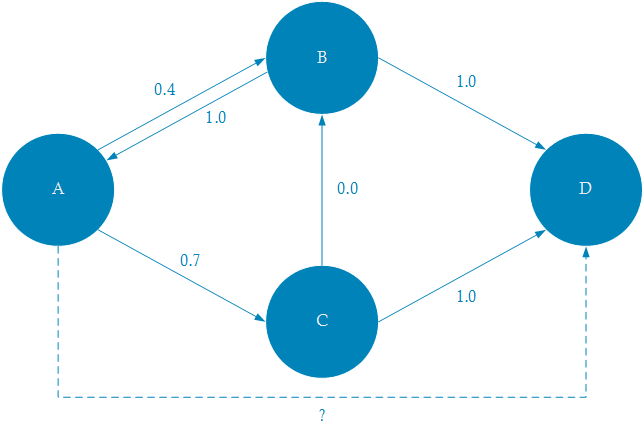
\includegraphics[width=2in]{image/webofTrust.png}
    \centering
    \caption[Trust Network]{Trust Network. Nodes are users and solid edges are trust statements. The dotted edge is one of the undefined and predictable trust statements (Adopted from \cite{Massa2004})}
    \label{figure:weboftrust}
\end{figure}

In addition to the trust network we will also have a rating matrix of size
$CxS$, where $S$ is the number of items. This rating will not differ from a
standard rating matrix, which are used in traditional collaborative filtering
systems. The value $u(c,s)$, is the rating given by user $c$ to item $s$, the
rating scale may differ from system to system.

% Architecture
The systems takes as input the trust network and the ratings matrix and
produces, as output, a matrix of predicted ratings that the users would assign
to the items. Figure \ref{figure:trustarchictecture} shows a conceptual
overview of the trust-aware recommender system architecture.

\begin{figure}[H]
    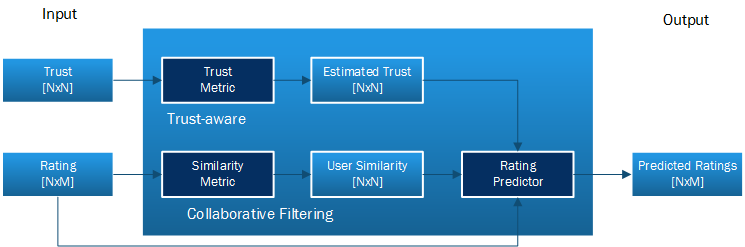
\includegraphics[width=5in]{image/trustawarearchitecture.png}
    \centering
    \caption[Trust-Aware Recommender System Architecture]{Trust-Aware
    Recommender System Architecture (Adopted from \cite{Massa2004})}
    \label{figure:trustarchictecture}
\end{figure}

The \emph{Trust Metric} module takes the trust network as input, and exploits
trust propagation in order to predict, for every user, how much she could trust
other users. Trust metrics can either be local and global. Global trust metrics
produces an estimated trust matrix with all the rows equal, meaning that the
estimated trust in a certain user (column) is the same for every user (row). A
simple local trust metric could e.g. for each user assign to every other user a
predicted trust based on her minimum distance from the source user. 

Massa et al. \cite{Massa2007} experimented with both local and global trust
metrics. The PageRank algorithm was used as a global trust metric. PageRank
tries to infer the authority of every single user by examining the structure of
the network. The algorithm follows a simple idea: if a link from user $A$ to
user $B$ represent a positive vote casted by $A$ to $B$, then the global rank
of a page depends on the number (and quality) of the incoming links. The trust
values assigned by users to users are used to predict the trustworthiness of
unknown users. Their findings, did not surprisingly, indicate that Global Trust
Metrics are not suited for the task of finding good neighbors, especially for
providing personalized recommendations, but is more suited for applications such
as \emph{Ebay.com} or similar to detect untrustworthy users. For their local trust metric
they used \emph{MoleTrust}, which is a depth-first graph walking algorithm with a tunable
trust horizon which allowed them to experiment with different propagation
distances. They found trusted users to be good predictors, especially for cold-start
users and they achieved a 63\% boots in prediction accuracy over traditional collaborative filtering
methods.

The \emph{Similarity Metric} module computes the user similarities, this is one
of the standard steps of any traditional collaborative filtering technique.

The \emph{Rating Predictor} can use the neighbors from the user similarity
matrix, the estimated trust matrix or a combination of both in order to
calculate the predicted ratings.

% Using a Trust Network to Improve Top-N Recommendation
Jamali et al. \cite{Jamali2009} propose two different methods for getting
around the cold-start user problem using a trust network. Their first approach
called \emph{Random Walk} only utilize the trust network to provide
recommendations. Starting from the active user $u$, one perform a random walk on
the trust network. Each random walk stops at a certain user. Then the items
rated highly by that user will be considered as recommended items, ordered
according to the ratings expressed by that user. Several random walks are
performed to gather more information and compute a more confident result. The
estimated rating of each item is the average of ratings for that item over all
raters considered. At the end, we output items with the highest estimated
rating as top-N recommended items. Their second approach called \emph{Combined
Approach} uses both user-user similarities and the trust network to provide
recommendations. In this approach we compute the top $K$ trusted users in the
network and rank the items rated by these trusted users to compute top-N
recommended items. The top $K$ trusted users can either be found by
\emph{Breadth First Search} or \emph{Random Walk in the social network}. We use
the collaborative filtering approach to compute another set of top-N
recommended items. Finally, we merge these two lists to produce a combined list
of top-N recommended items. Items returned by CF is denoted as $CF_{u}$, while
the items returned by Trust-based approach are denoted $TR_{u}$.

\begin{equation}
 \hat{u}(c,s) =
  \begin{cases}
   \frac{u_{tr_{c,i}}+u_{cf_{c,i}}}{2}     & i \in TR_{u};i \in CF_{u}         \\
   \hat{u_{tr_{c,i}}}                      & i \in TR_{u};i \not \in CF_{u}    \\
   \hat{u_{cf_{c,i}}}                      & i \in CF_{u};i \not \in TR_{u}     \end{cases}
\end{equation}

The top-N items with the highest value of $\hat{u}(c,s)$ will be returned as
the top-N recommended items. The authors also experimented with weighted
averaging in the case where the item appear in both $TR_{u}$ and $CF_{u}$.
Their approaches showed great improvements in recall for cold-start users,
improving the performance by 50\% over standard CF methods. The main
improvements however, are the coverage of the trust-based approaches, while
still maintaining the same or even slightly better precision than the standard
CF methods.

Papagelis et al. \cite{Papagelis2005} proposed to alleviate sparsity using
trust inferred from user-user similarity. This approach does therefore not
require users to explicitly express their trust in other
approaches described above, the trust information is inferred from the
underlying social network of the rating matrix. Their approach is based on the
assumption that the more similar two users are, the greater their established
trust would be considered.

\begin{figure}[H]
    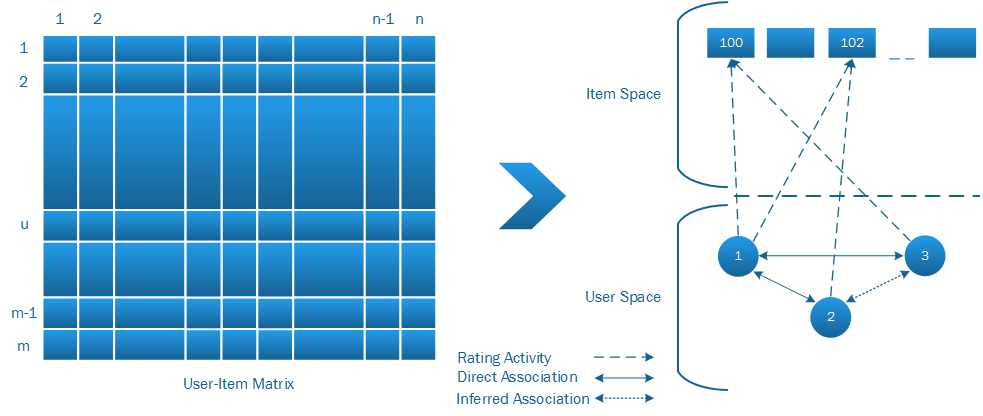
\includegraphics[width=5in]{image/trustnetwork.png}
    \centering
    \caption[Underlying Social Networks in Recommender Systems]{Underlying Social Networks in Recommender Systems}
    \label{figure:cfsocialnetwork}
\end{figure}

Due to the number of ratings that exist in recommendation systems, underlying
social networks are very sparse. There are cases in which insufficient or loss
of information is detrimental for the recommendation algorithms. Consider
Figure \ref{figure:cfsocialnetwork}, classic CF will associate only the users
which have co-rated an item (User $1$ and $2$ and user $1$ and $3$). To deal
with the problem of a sparse social network, it is possible to infer trust
between a source user $S$ and a target user $T$ through an intermediate user
$N$ (User $2$ and $3$ are connected through the intermediary user $1$), as
shown by the \emph{Inferred Association} arrow. According to this process,
trust is propagated in the network and associations between users are built,
even if they have no co-rated item. Trust paths can be of variable length,
depending on the number of associations that one needs to traverse in order to
reach the target user.

% Trust-paths
For example, if the trust $t_{(1,2)} = 0.7$ based on 5 co-rated items
and $t_{(1,3)} = 0.35$ based on 2 co-rated items, then the trust
between user $2$ and $3$ through $1$ is, $\frac{0.7*5}{5+2} + \frac{0.35*2}{7} = 0.6$.

In order to express the subjective notion of trust, the authors set up a
confidence model that is assigned to each direct association of the network
that expresses the reliability of the association. Confidence is related to the
number of co-rated items between two users. The confidence scores are all
expressed in relation to the most confident association for each user.

\begin{equation}
c_{(s,t)} = \frac{n(I_{s} \cap I_{t})}{n(I_{s} \cap I_{u_{MAX_CONF}})}
\end{equation}

Using the above example, assuming that the maximum number of co-rated items
user $1$ has with any user is 7, $c_{(1,2)} = \frac{5}{7}$.

% Results/Findings
The authors achieved improved accuracy for all sparsity levels. With a sparsity
level of $99.9\%$ the 2-HOP CF (friend of friends) increased the MAE
performance by $17\%$ over standard CF methods.

Victor et al. \cite{Victor2008} points out that cold-start users not only have
expressed few ratings, but also typically have expressed trust in few users. In
order for trust-aware recommenders to help cold-start users they need to have
expressed trust in at least one user. But choosing who to connect to is often a
difficult task. To help cold-start users find trusted users, Victor et al.
propose using key figures or mavens (users who write many reviews), frequent
raters (users who evaluate many items) and connectors (users with
many trust connections). By connecting to these key figures, cold-start users
shown a significant increase in coverage while still maintaining good accuracy.
They also show that connecting to key figures are more beneficial to a
cold-start user than connecting to a random user.

\subsection{Filterbots}

% Na¨ıve Filterbots for Robust Cold-Start Recommendations

Park et al. \cite{Park2006} propose using filterbots to improve the cold-start
performance of collaborative filtering methods. Their filterbots are a varition
of RipperBots, described in detail in \cite{Good1999}. A filterbot is an
automated agent that rates all or most items using information filtering (IF)
techniques. The filterbots injects psuedo users or bots into the system. These
bots rate items algorithmically according to item features and user profiles.
For their movie recommendation systems the authors used 7 global bots which
e.g. rated movies based on average item rating, a critic bot that generates ratings
based on the average critic (pre-selected users) ratings, an award bot that
generates rating based on the awards a movie has won, and so on. These ratings
generated by these bots are injected into the user-item matrix along with
actual user-item ratings. Standard CF algorithms are then applied to generate
recommendations.

Their approach clearly demonstrated better robustness to all three cold-start situations than standard item-based
and user-based collaborative filtering. The improvements were most evident on
the datasets with a high degree of sparsity.

\subsection{Wisdom of the better few / Seed users}

% Wisdom of the Better Few: Cold Start Recommendation via Representative based Rating Elicitation

Liu et al. \cite{Liu2011} propose an approach in which they elect a few
representative users and items. The representative set should represent a set
of active users or items who well represent the entire population but with
little taste overlap. In their approach they wish to find a rank-k
factorization of the form $Y \approx XR$ or $Y \approx CX$ where $X$ is a
loading matrix consisting of free parameters and $R$ and $C$ which is the
component matrix consisting of actual rows or columns from $Y$. The
representative users and items are found using dimensionality reduction
techniques by reducing the column space of the rating matrix from $m$ to $k$.
And then applying basis selection based on the maximum-volume principle to
select the $k$ most representative users or items. In order to be able to
recommend new items to the users it must first be rated by the $k$
representative users, likewise for new users to be rated they need to rate the
$k$ most representative items. Their method therefore allows new users
and items to be \emph{folded in}.

\subsection{Intelligent Selection / Interview Process}\mbox{}\\

\begin{chapquote}[30pt]{Vanessa Redgrave}
  "Ask the right questions if you're going to find the right answers"
\end{chapquote}

% Getting to Know You: Learning New User Preferences in Recommender Systems

As pointed out by Rashid et al. \cite{Rashid2002}, the most direct way of
acquiring information for use in personalized recommendations from a new users
is to present item for the user to rate. However, they argue that the system
must be careful to present useful items to garner information. A fashion
recommender should probably not ask whether a new user likes any \emph{essential}
items as most users already have these items in their wardrobe. Therefore, knowing
that a new user likes an \emph{essential} item tells you very little about
the user. The choice of what questions to ask a new user, then, is critical.
The authors performed a study of different item selection strategies that collaborative
filtering recommender systems can use to learn about new users. They presented the users
with a questionnaire with items asking them to rate/select the ones they like.
Their strategies can be divided into five classes, which they evaluated based
on user effort and accuracy:

\begin{itemize}
\item Random: strategies: Strategies that avoid bias in the presentation
	  of bias
\item Popularity: Select among the top N items where the probability
	  that an item is selected is proportionate to the items popularity.
\item Pure entropy: Present the items with the highest entropy that the
	  user has not seen
\item Balanced strategies: A balanced approach combining both popularity
	  data and entropy.
\item Personalized: As soon as some information is known about a user,
	  present items specifically tailored to that user using e.g. item-item
	  similarity
\end{itemize}

The authors found Popularity and balanced strategies to perform the best. Their
recommendation for an e-commerce recommender is to start recommending the most
popular items, rather than the highest rated ones, and then use item-item
strategies to personalize the recommendations as quickly as possible. The same
study was later extended by Rashid et al. \cite{Rashid2008} where they more
closely examined information theoretic strategies for item selection. In the
article they introduced three new strategies, which again was evaluated based
on user effort and accuracy:

\begin{itemize}
\item Entropy0: Entropy Considering Missing Values
\item HELF: Harmonic mean of Entropy and Logarithm of Frequency
\item IGCN: Information Gain through Clustered Neighbors
\end{itemize}

The authors point out that popularity based approaches are likely to worsen the
\emph{prefix-bias}, meaning that popular items garner even more evaluations.
The accuracy differences between the approaches is fairly small, IGNC performed
the best closely followed by Entropy0 and Popularity. However, the expected
utility of the profiles built using popularity is much lower than the ones built
using information theoretic approaches.\newline

% User effort vs. accuracy in rating-based elicitation
The question then, is how many items you should ask a user to rate. Cremonesi
et al. \cite{Cremonesi2012} performed a set of experiments where they looked
at the trade-off between user-effort and accuracy. More specifically, how many
ratings are enough to provide good quality recommendations to new users? The
authors concluded that between 5 and 20 ratings are optimal for the movie
domain and that that 10 ratings is generally \emph{enough}, but that this number
depends on the recommendation method and the dataset used.

\subsection{Hybrid Methods}

Another line of search for solving the cold-start problem is to utilize
features of items and users. The content features can be used to capture the
similarities between users and items, thus reducing the amount of data required
to make accurate predictions. User data that may be collected typically
includes age, gender, nationality, marital status, income, educational level
and occupation. Item data could e.g. be the price of a product, title,
description, editorial ratings and so. The idea is that people with a more
common background share a more similar taste than someone with a random
background, and therefore good recommendations can be made as long as we know
something about the new user's background.

This section will present some latent factor models presented recently proposed
that incorporate both user/item features in addition to user-item interactions.
In Matrix factorization methods, the regularization is mostly based on a
zero-mean Gaussian prior on the factors, we refer often referred to as
ZeroMean. However in the following models the dyadic response matrix $Y$ is
estimated by a latent factor model such that $Y \approx U^{T}V$, where the
latent factor matrices, $P$ and $Q$, are estimated by regression such that $P
\approx FX$ and $Q \approx MZ$. $X$ and $Z$ denote user attribute and item
feature matrices, and $F$ and $M$ are weight matrices learned by regression.
The main difference between the following methods is how they estimate these
weight matrices.

% Regression-based Latent Factor Models

Agarwal et al. \cite{Agarwal2009} propose a class of latent factors models
called regression-based latent factor model (RLFM) that incorporates both
user/item features and past interaction data into a single model. Their
approach utilizes features of items and users as the prior distribution for
latent profiles in matrix factorization. Regularizing latent factors through
regression has important consequences when modeling sparse dyadic data. For
users/items with little data, one obtain reliable factor estimates by using the
regression estimates as a fallback. This allows the model to effectively deal
with both cold start and warm start situations. Their method assumes a Gaussian
prior, but replaces the zero mean with a feature-based regression, thus it
simultaneously regularizes both user and item factors through known features.
Users and items are anchored around a global feature-based one where profiles
are constructed by estimating deviations from the global ones in a smooth
fashion. The deviation depends on the amount of information available, e.g.
items/users with sparse data are aggressively "shrunk" to the global one. New
items and users start out with profiles based on their known features that gets
refined smoothly with the availability of more data. The model also supports
dynamic updates, which gives more weight to recent data. Their proposal is a
batched online learning scheme which updates the model on fixed time intervals
or after a predetermined amount of new observations have been made.

Their model outperformed all other models on both the MovieLens and EachMovie
datasets, and their dynamic model in particular significantly outperformed all
other models.

% fLDA: Matrix Factorization through Latent Dirichlet Allocation

Agarwal et. al \cite{Agarwal2010} propose a Matrix factorization method to
predict ratings in recommender system applications where a "bag-of-words"
representation of item meta-data is natural. Their method regularizes both user
and item factor simultaneously through user features and the bag of words
associated with each item. The key idea of their method is to let user factors
take values in an Euclidean space of existing factorization models, but assign
item factors through a richer prior based on Latent Dirichlet Allocation (LDA).
The main idea behind LDA is to attach a discrete latent factor to each word of
an item that can take $K$ different values ($K$-topics) and produce item topics
by averaging the per-word topics in the item. An article where 80$\%$ of the
words are assigned to politics and the rest to education would be though of as
a political article related to the issue of education. This allows us to model
the affinity between user $i$ and item $j$ as $s'{j}\hat{z_{j}}$, where
$\hat{z_{j}}$ is the multinomial probability vector representing the soft
cluster membership score of of item $j$ to the $K$ different latent topics.

% Matchbox: Large Scale Bayesian Recommendations
%   Online algorithm

Stern et al. \cite{Stern2009} presents a probabilistic model called Matchbox.
The system makes use of content information in the form of user and item
meta-data in combination with collaborative filtering information from previous
user behaviour in order to predict the value of an item for a user. Much like
\cite{Agarwal2009} the factors are regularized by incorporating more
flexibility in the Gaussian priors through regression on user and item factors.
Their model is dynamic, meaning that it allows an item's popularity, a user's
taste or user's personal rating scale to drift over time, as well as having the
option to be trained incrementally using Assumed Density Filtering (ADF). This
means that the value of weight matrices $F$ and $M$ will drift over time, this
is accomplished by the addition of Gaussian noise each time step. Inference is
accomplished a combination of message passing and expectation propagation.

The authors show that they can achieve state-of-the-art performance when
training the model in an on-line manner, which is especially beneficial for
dynamic domains where it is important to always have an up to date model.
Matchbox was able to train the model for the Netflix Dataset in about 2 hours
using 8 cores, meaning that it is able to add up to 14000 ratings per second.
These methods also provide quick recommendations, which is important in an
online applications, the system was able to generate 2,500,000 recommendations
in 0.25 seconds using Approximate KD Trees.

% Learning Attribute-to-Feature Mappings for Cold-Start Recommendations
%   Model for positive implicit feedback!
%   Demonstrates usefulness for new-item recommendations
%   See A. Item Recommendation from Implicit Feedback in the article for implicit feedback recommendations
%   k-NN worked best with MORE features than the linear mapping functions
%   Code can be found at: ismll.de/mymedialite

Gantner et al. \cite{Gantner2010} propose a method on how to map additional
information such as user and item features to the latent features of a matrix
(or higher dimensional) factorization model. At the core of their approach is a
standard factorization model, optimized to the recommendation task. The
extensions include a mapping function that compute adequate latent
representations for new entities from their attribute representations. This
mapping function could allow new items and users latent features to be found
only based on content-information and further on be used as if they were
normally trained latent features. The training of the factorization model with
a mapping extension consists of the following steps:

\begin{enumerate}
\item Training the factorization model using the data $S$, and then
\item Learning the mapping functions from the latent features of the entities
\end{enumerate}

The authors use BPR-MF, a matrix factorization model based on the Bayesian
Personalized Ranking (BPR) framework as their factorization model. The authors
experimented with two different ways of mapping item/user attributes to the
factor space (Only attribute-to-feature mapping for items are presented in the
article):

\begin{enumerate}
\item k-NN Mapping: Weighted k-NN regression for each factor. Determine the
k-nearest neighbors as the most similar items according to the cosine
similarity of the attribute vectors.
\item Linear Mapping: Each item factor is expressed by a weighted sum of the
item attributes. Suitable parameters for the mapping function is learned by
optimizing the model for the squared error on latent features.
\end{enumerate}

The authors found that linear mapping worked the best, and that their method
yields accuracy comparable to state-of-the-art methods.

\subsection{A Discussion on the Cold-start Solutions}
\ref{sec:cold-start-discussion}

The following discussion will be based on the following points: the user-effort
required before the system can start providing high quality recommendations, the
cold-start performance of the system, how well the method fits our application
and whether or not it is a good match for our specific domain.

\subsubsection{Trust-aware recommenders}

%How can this be implemented in our system?
Requiring users to explicitly express trust, is not something users necessarily
will frown upon. Services like Instagram, Facebook and many others offers a
\emph{follow} function to their users, filling their news feeds with content from
the users which they have chosen to follow. For SoBazaar we imagine that you
e.g. could chose to follow people either because they have a good taste in
clothes or that you simply are friends, and you want to keep up with what your
friends are buying. We believe that the \emph{follow user} functionality, is
a \emph{frictionless} way of collecting high quality user information.

As previously mentioned finding trusted users can be hard. Meaning that the
application itself must be adapted to make it easy to find friends (e.g. from facebook)
which they can choose connect to. Other ways of finding users to connect to might
include \emph{most followed} users or something similarly.

As previously mentioned Massa et. al. \cite{Massa2007} found trusted users
to be good predictors. Looking directly at trusted users improved the
predictive accuracy by 62\% over traditional collaborative filtering methods
for cold-start recommendations. E.g. by using the methods described by
Jamali et. al. \cite{Jamali2009} these methods could be combined with a traditional collaborative
filtering based system to improve recommendation quality. Massa et al. \cite{Massa2004} also argue that it is more
useful for a recommender system to ask for one trust statement than asking for
one rating for new users, making it a good potential solution to the cold-start
problem given that new users of the application easily can find friends
to connect to when first using the application.

We believe trust-aware recommenders to be a good fit for the application
due to its \emph{social nature}. We believe that trust aware recommender systems
is something that should be considered at a later point when more social functionality
is in place, to further enhance the recommendation quality
 
\subsubsection{Interview Process}

%How can this be implemented?
Our rational behind including these articles is that we envision a simple "hot
or not" tinder like interface to be presented when new users log into the system.
You can then ask the user to "rate" e.g. 10 items by quickly \emph{swiping} them
left or right. However, requiring the user to rate rate a certain amount of items
can also be \emph{dangerous}. One should therefore perform a user study or similar
to see how users experience this feature. We also imagine that the tinder interface
could be available as a feature in the application for users users who just want a 
fun way of browsing clothes on their mobile phone. If done right this can be
a great feature for collecting large amounts of both positive and negative feedback
from the users.

An important question to answer is how this interface will select items to 
present to the user. One could either choose the simple approach of
recommending the most popular items to the user, but as previously mentioned
this is likely to worsen the prefix bias. Rashid et al. \cite{Rashid2008} got
the best results using information theoretic approaches and argues that simpler
methods such as most popular is likely to worsen the prefix bias. The authors
found Information Gain through Clustered Neighbours (IGCN) to have the best
performance overall, which they gave a maximum score for its accuracy. We choose
to ignore their user effort dimension as rating movies and clothes are two
completely different things. In order to rate a movie you must have watched
it, when it comes to clothes a quick glimpses of the item is enough.
A third strategy could be to present the newest or \emph{freshest} items
making it a fun way for users to explore the newest additions.

%Scalability & Final Verdict
We really like this approach as it is simple and elegant. Having this
functionality would make the number of user feedback available sky-rocket in addition
to providing high quality explicit feedback that is both positive and negative.
By incorporating some smart way of selecting the items which are presented
one could find ways to garner ratings for large portions of the item collection
or collecting preference data quickly about new items. However, we believe
that having negative feedback is one of the strongest arguments for applying
this method. The negative aspects of this approach is mainly limited to the fact
that it requires some active user involvement.

\subsubsection{Seed users}

In our opinion, this approach is not that suited for our domain, as it fairly
dynamic and we are working with a large and dynamic item collection. For an item to be
recommendable it must be rated by all representative users, which is highly
unlikely given the size of the item collection itself. E.g. if we have e.g. 20, 40 or 100
representative users and a spring collection is launched containing 6000 items,
for all these items to be recommendable these 15 representative users must rate
all these items. However, this method does shows some promise as a selection criteria
for items to ask the user to rate for a interview process.

\subsubsection{Filterbots}

Filterbots is a simple, but elegant solution to the cold-start problem first
presented in 1998 by Sarwar et. al. \cite{Sarwar1998}. This method
requires no user-effort other than requiring the user to rate at least one
item before recommendations can be made. 
Park et al. \cite{Park2006} clearly demonstrated the robustness of their Naive
Filterbot compared to item-based and user-based approaches in all three
cold-start scenarios. The results in \cite{Agarwal2009, Agarwal2010} also show
that the Naive Filterbots are very close to the state-of-the-art
latent factor models in terms of performance for all sparsity levels.

Filterbots could easily be implemented in any system as it only requires
the data to be run through an additional preprocessing step before it
is used to train the model. It is worth that filterbots were developed
for neighborhood models, and you can not expect getting the same kind
of performance improvements using latent factor models.

To incorporate filterbots in our system we would first have to define what filterbots
we wound want to use and what we want to achieve be using them. E.g. by using multiple
brand bots that gives each item of a certain brand a max score would make it possible to give brand specific
recommendations as soon as a user have expressed preferences for an item, thus connecting
him to a filterbot with high ratings for all items of the given brand. Similarly
a \emph{PopularityBot} would \emph{recommend} the most popular items to users which
they are connected to. These bots can therefore be made to capture the general underlying
trends of the users or give recommendations based on content-features of the items.
Given that we use the bots mentioned above, as soon as a new user rates a single item
rated by both bots he would theoretically be recommended the most popular items of
the brand which she expressed her preference for, making it a potentially good fit for fashion
recommendations.

\subsubsection{Hybrid recommenders}

%TODO - Summarize results
Latent factor models are currently the main paradigm within the recommender
system field and are currently considered the state-of-the-art recommendation
methods. The all the hybrid methods achieved state-of-the-art performance as well as
having good fallback methods based on user and item features to solve the
cold-start problem. In addition to incorporating item-features and/or user-features
these models also incorporate some notion of recency, reducing the importance of
items over time. Another advantage of these models are that they support
online training of the models, which further could improve the cold-start
performance by \emph{instantly} incorporating new preferences.

In order to implement these recommender we would first need access to
high quality item and user-features. The item-attributes could be extracted
from the product database, which demographic information could e.g. be
extracted from Facebook data. Another concern of ours is that our dataset is
currently to small for latent factor methods, since most of these methods
rely on binary data (e.g. purchases only) to provide recommendations.


\subsubsection{Summary}

It is hard to compare the performance of the different methods as the authors have
experimented with different datasets and evaluation measures making it hard to do
a quantitative comparison. We therefore opted to do qualitative assessment of the methods
in question. It is worth nothing that qualitative methods are less about attempting to prove
something than about to understand something. Our ordinal rating scale spans from \ding{55} meaning
\emph{bad}, \checkmark means \emph{good} \ding{55} and finally \checkmark\checkmark means \emph{best}


\begin{table}[H]
    \centering
    \begin{tabular}{*{4}l}
    \toprule
    Method					& Cold-start performance  & User-effort \\ 			\midrule
    Trust-aware RS 			& \checkmark			  &	\ding{55}				\\ 
    Filterbots 				& \checkmark			  &	\checkmark\checkmark	\\ 
    Seed users 				& \checkmark			  &	\ding{55}				\\ 
    Intelligent selection 	& \checkmark			  &	\checkmark				\\
    Hybrid Methods 			& \checkmark \checkmark	  &	\checkmark\checkmark	\\
    \bottomrule
    \end{tabular}
    \caption[Evaluation of cold-start methods]{Evaluation of cold-start methods}
    \label{table:evaluationcoldstart}
\end{table}

Trust-aware recommender systems get a \ding{55} in user effort as it is hard to find users to connect to,
this problem could however be mitigated by implementing a system like the one described by Victor et al. \cite{Victor2008}
to recommend users to connect to. Seed users also get a \ding{55} in user-effort, mainly due to its solution to the new item
problem where all representative users must rate an item for it to be recommendable. Filterbots and the Hybrid methods both
get two checkmarks for requiring no extra user involvement. Intelligent selection could pretty seamlessly be integrated into
the solution using e.g. a simple \emph{hot or not} interface, requiring minimal user effort. We would also like to argue that having the
option to incrementally update the model is an important feature which could further improve cold start performance, as it instantly can
incorporate the ratings given by new users and to new items. The hybrid methods therefore gets to checks for their cold-start performance.

From our discussion we believe filterbots, interview process and hybrid methods such as e.g. RBLF and MatchBox could provide good solutions.
However, we are currently limited to experiment with filterbots as we do not have access to user and item features or any way
of testing out an interview process.
